%!TEX root = report.tex

\section{Results}
It should be noted that all four algorithms are color-coded consistently throughout the plots. The lines represent averages of 10 training runs. The error bars are based on the standard error at that point in time. All tables are based on the final 2500 episodes of these 10-run averages.
\subsection{10-by-10 simulations}
% FIGURES 10-sized
\begin{figure}[H]
    \centering
    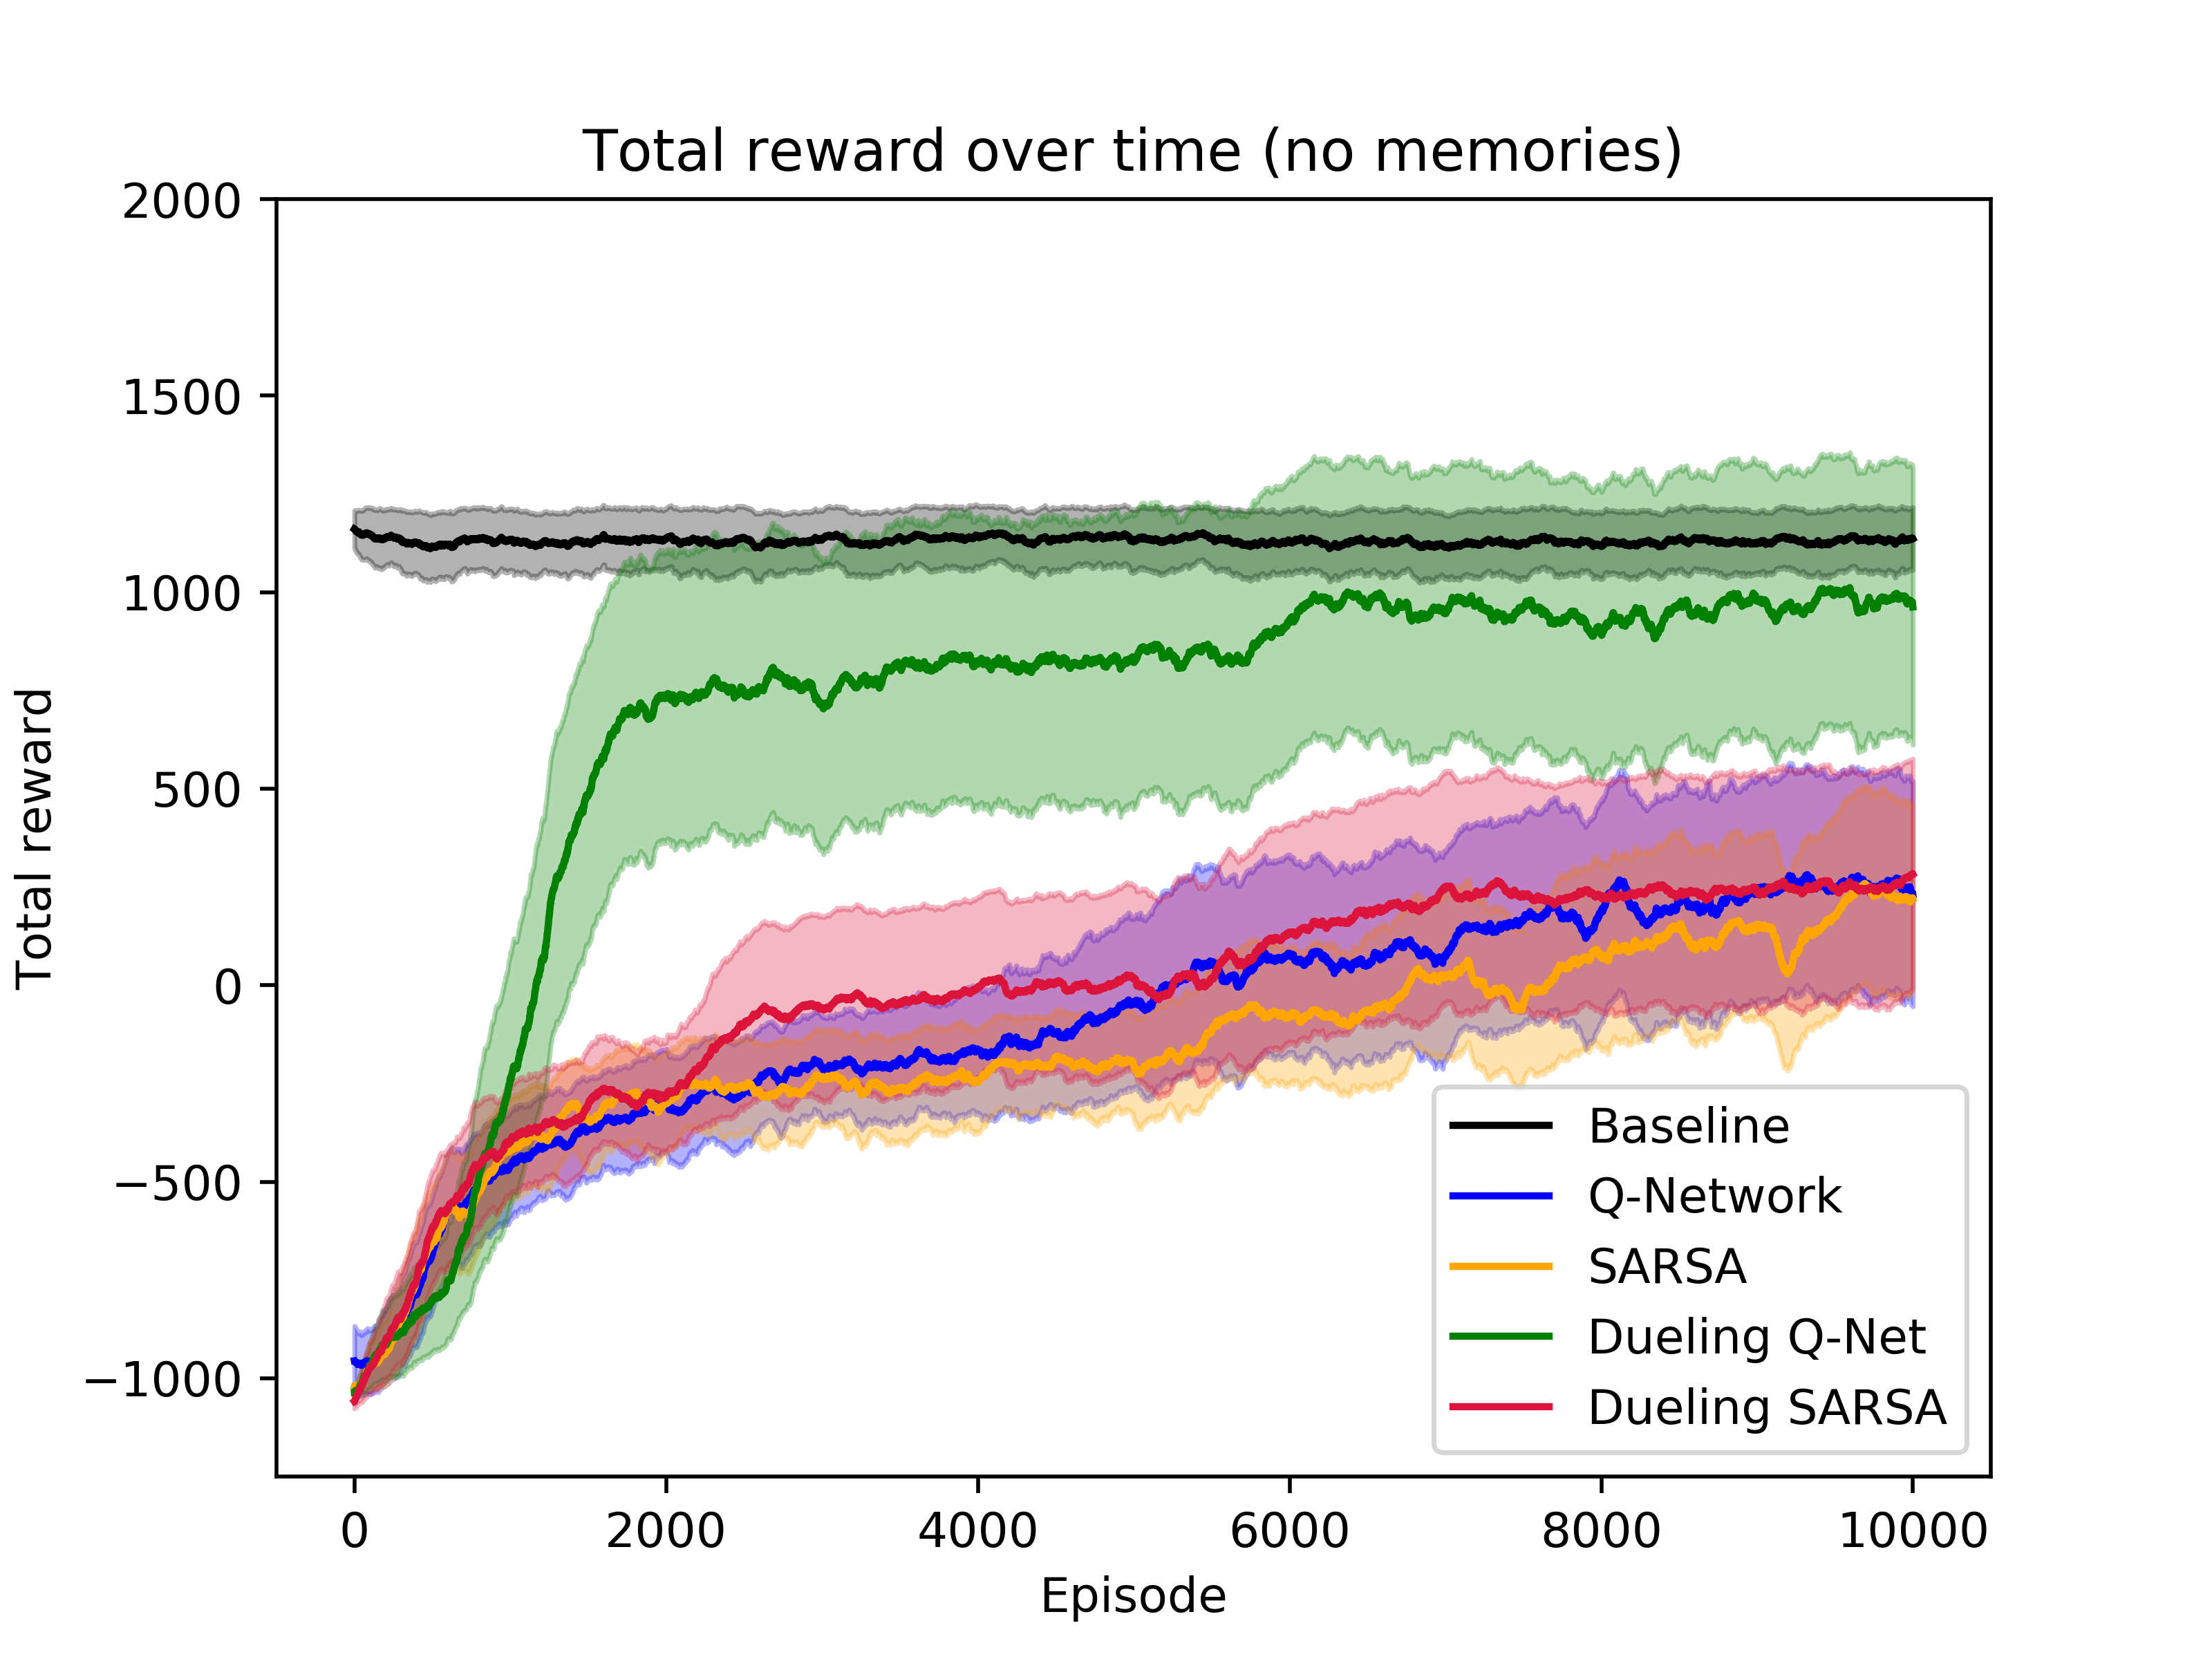
\includegraphics[width=\linewidth]{img/results/10-sized/total_rewards_0m-min.png}
    \caption{10-run averages given 0 episodes of demonstration data.}
    \label{fig:10sized-0mem}
\end{figure}
\begin{figure}[H]
    \centering
    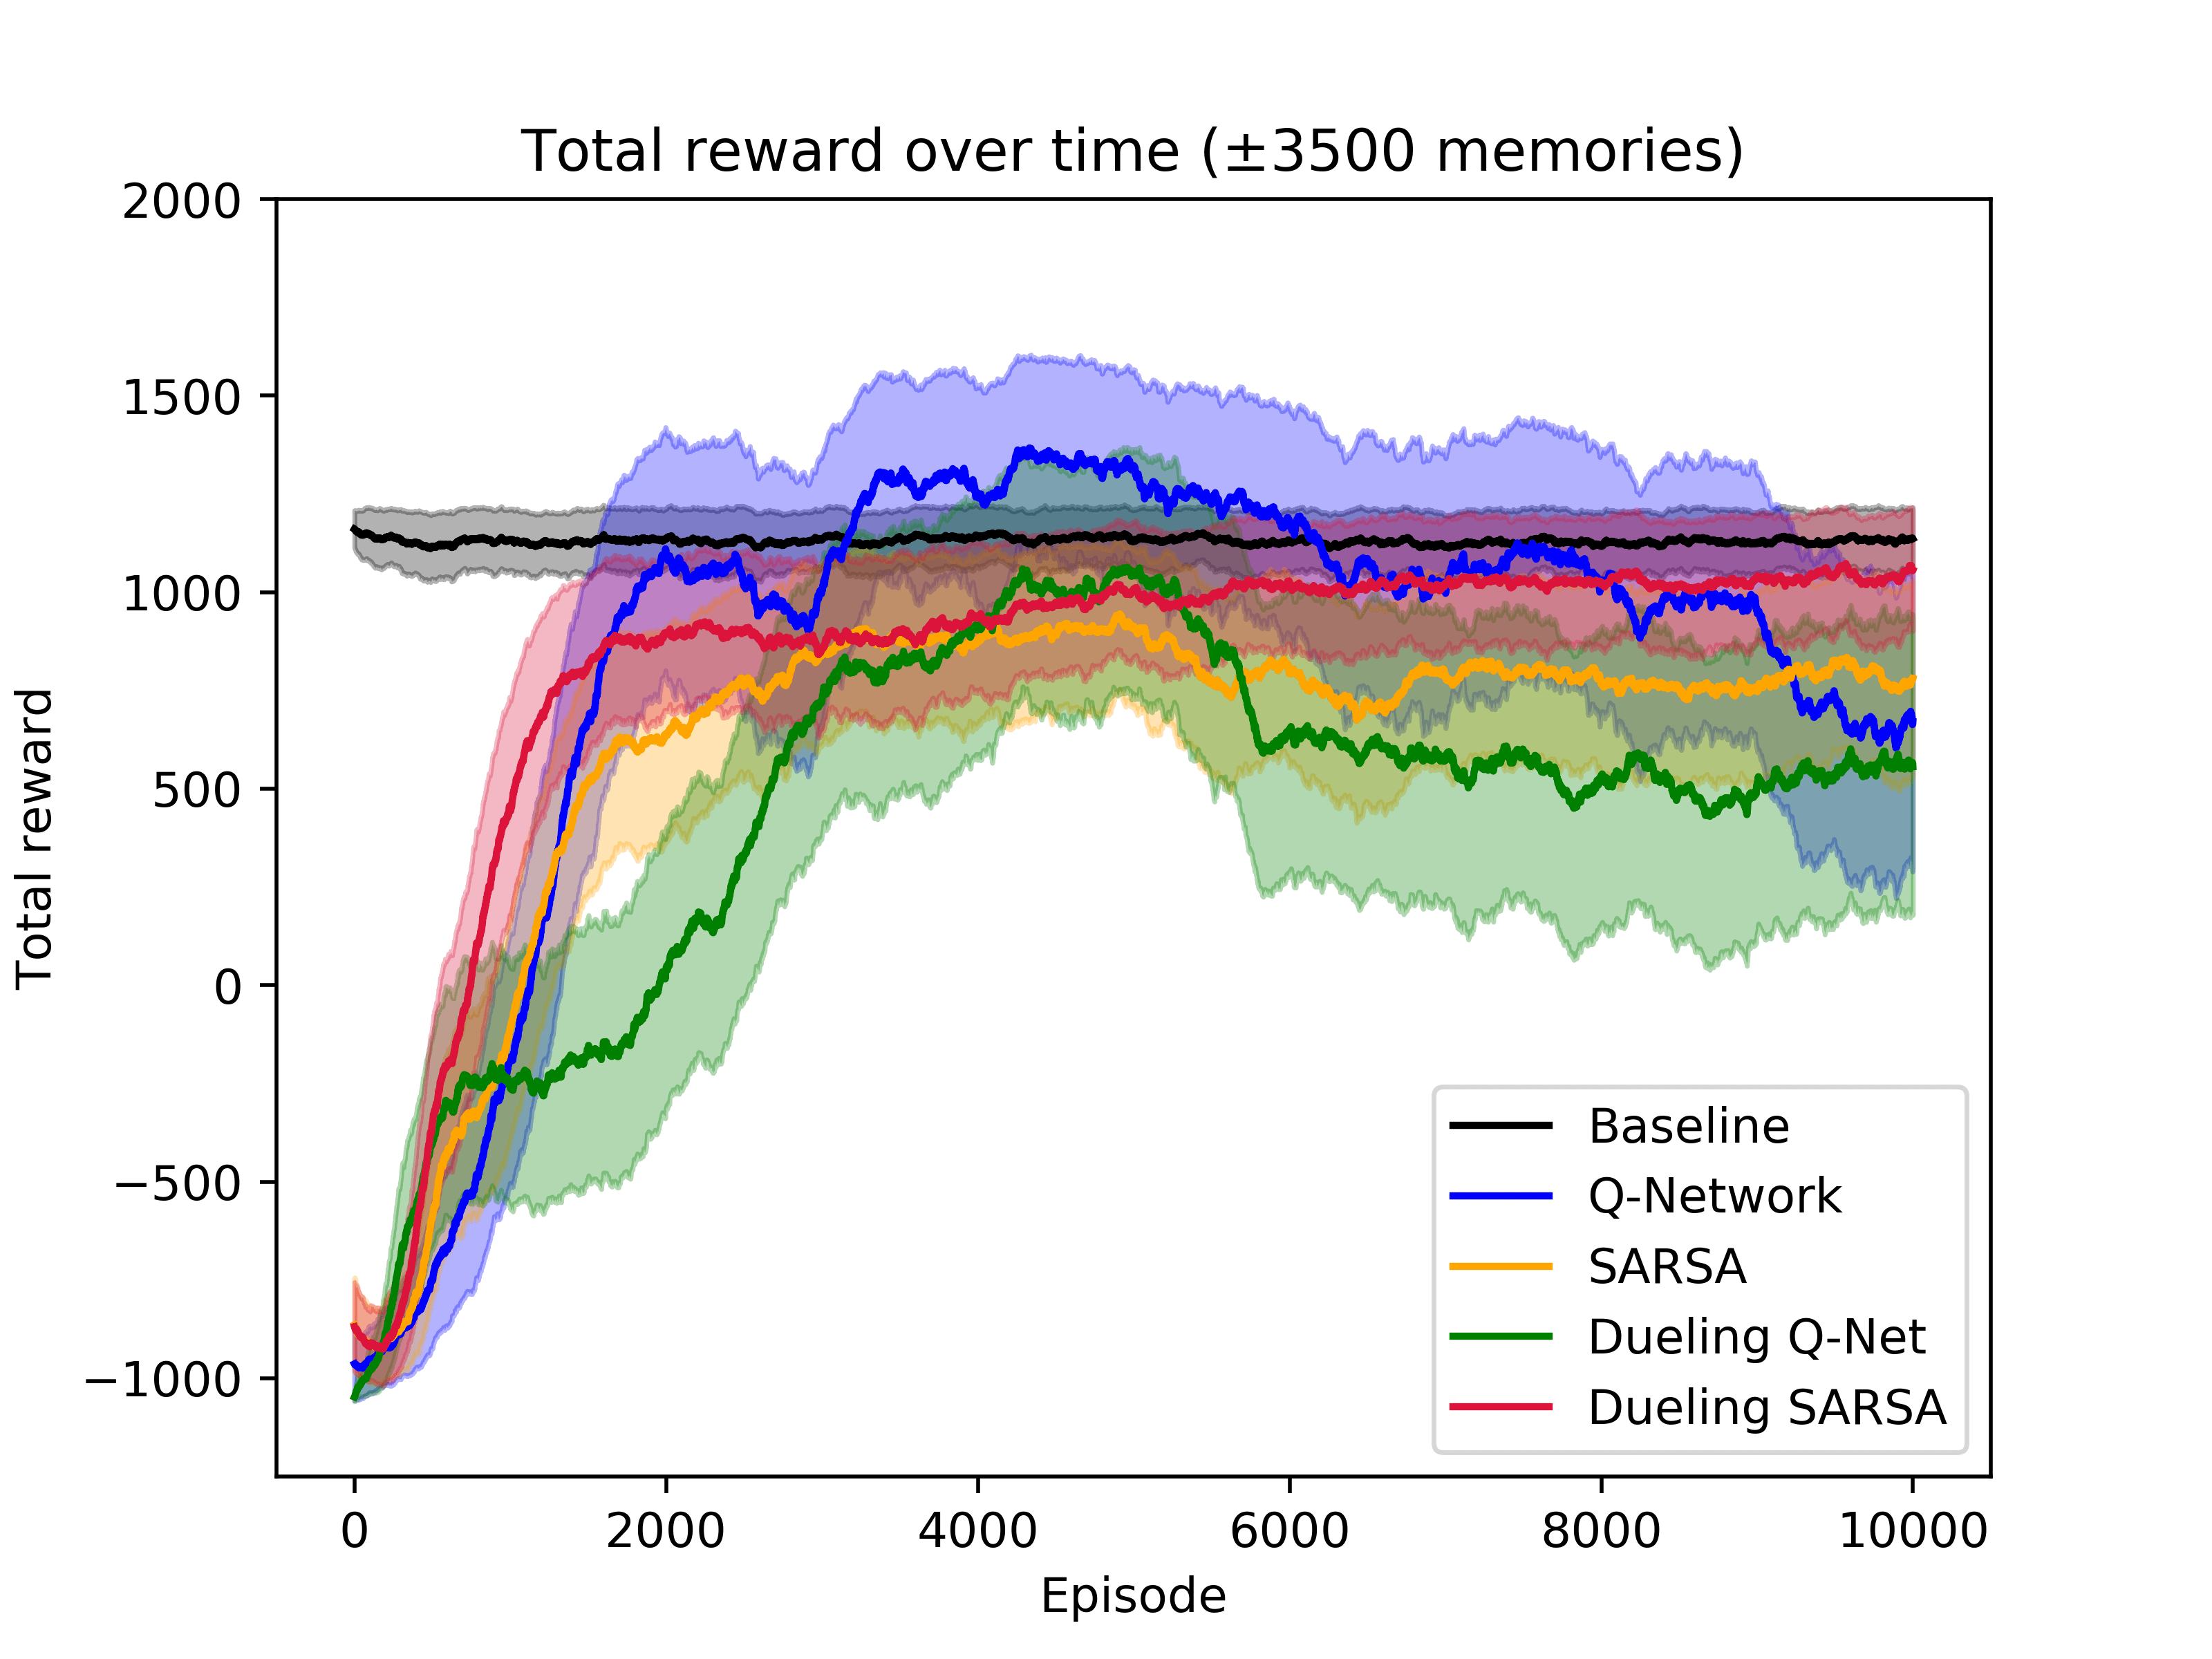
\includegraphics[width=\linewidth]{img/results/10-sized/total_rewards_100m-min.png}
    \caption{10-run averages given 100 episodes of demonstration data.}
    \label{fig:10sized-100mem}
\end{figure}
\begin{figure}[H]
    \centering
    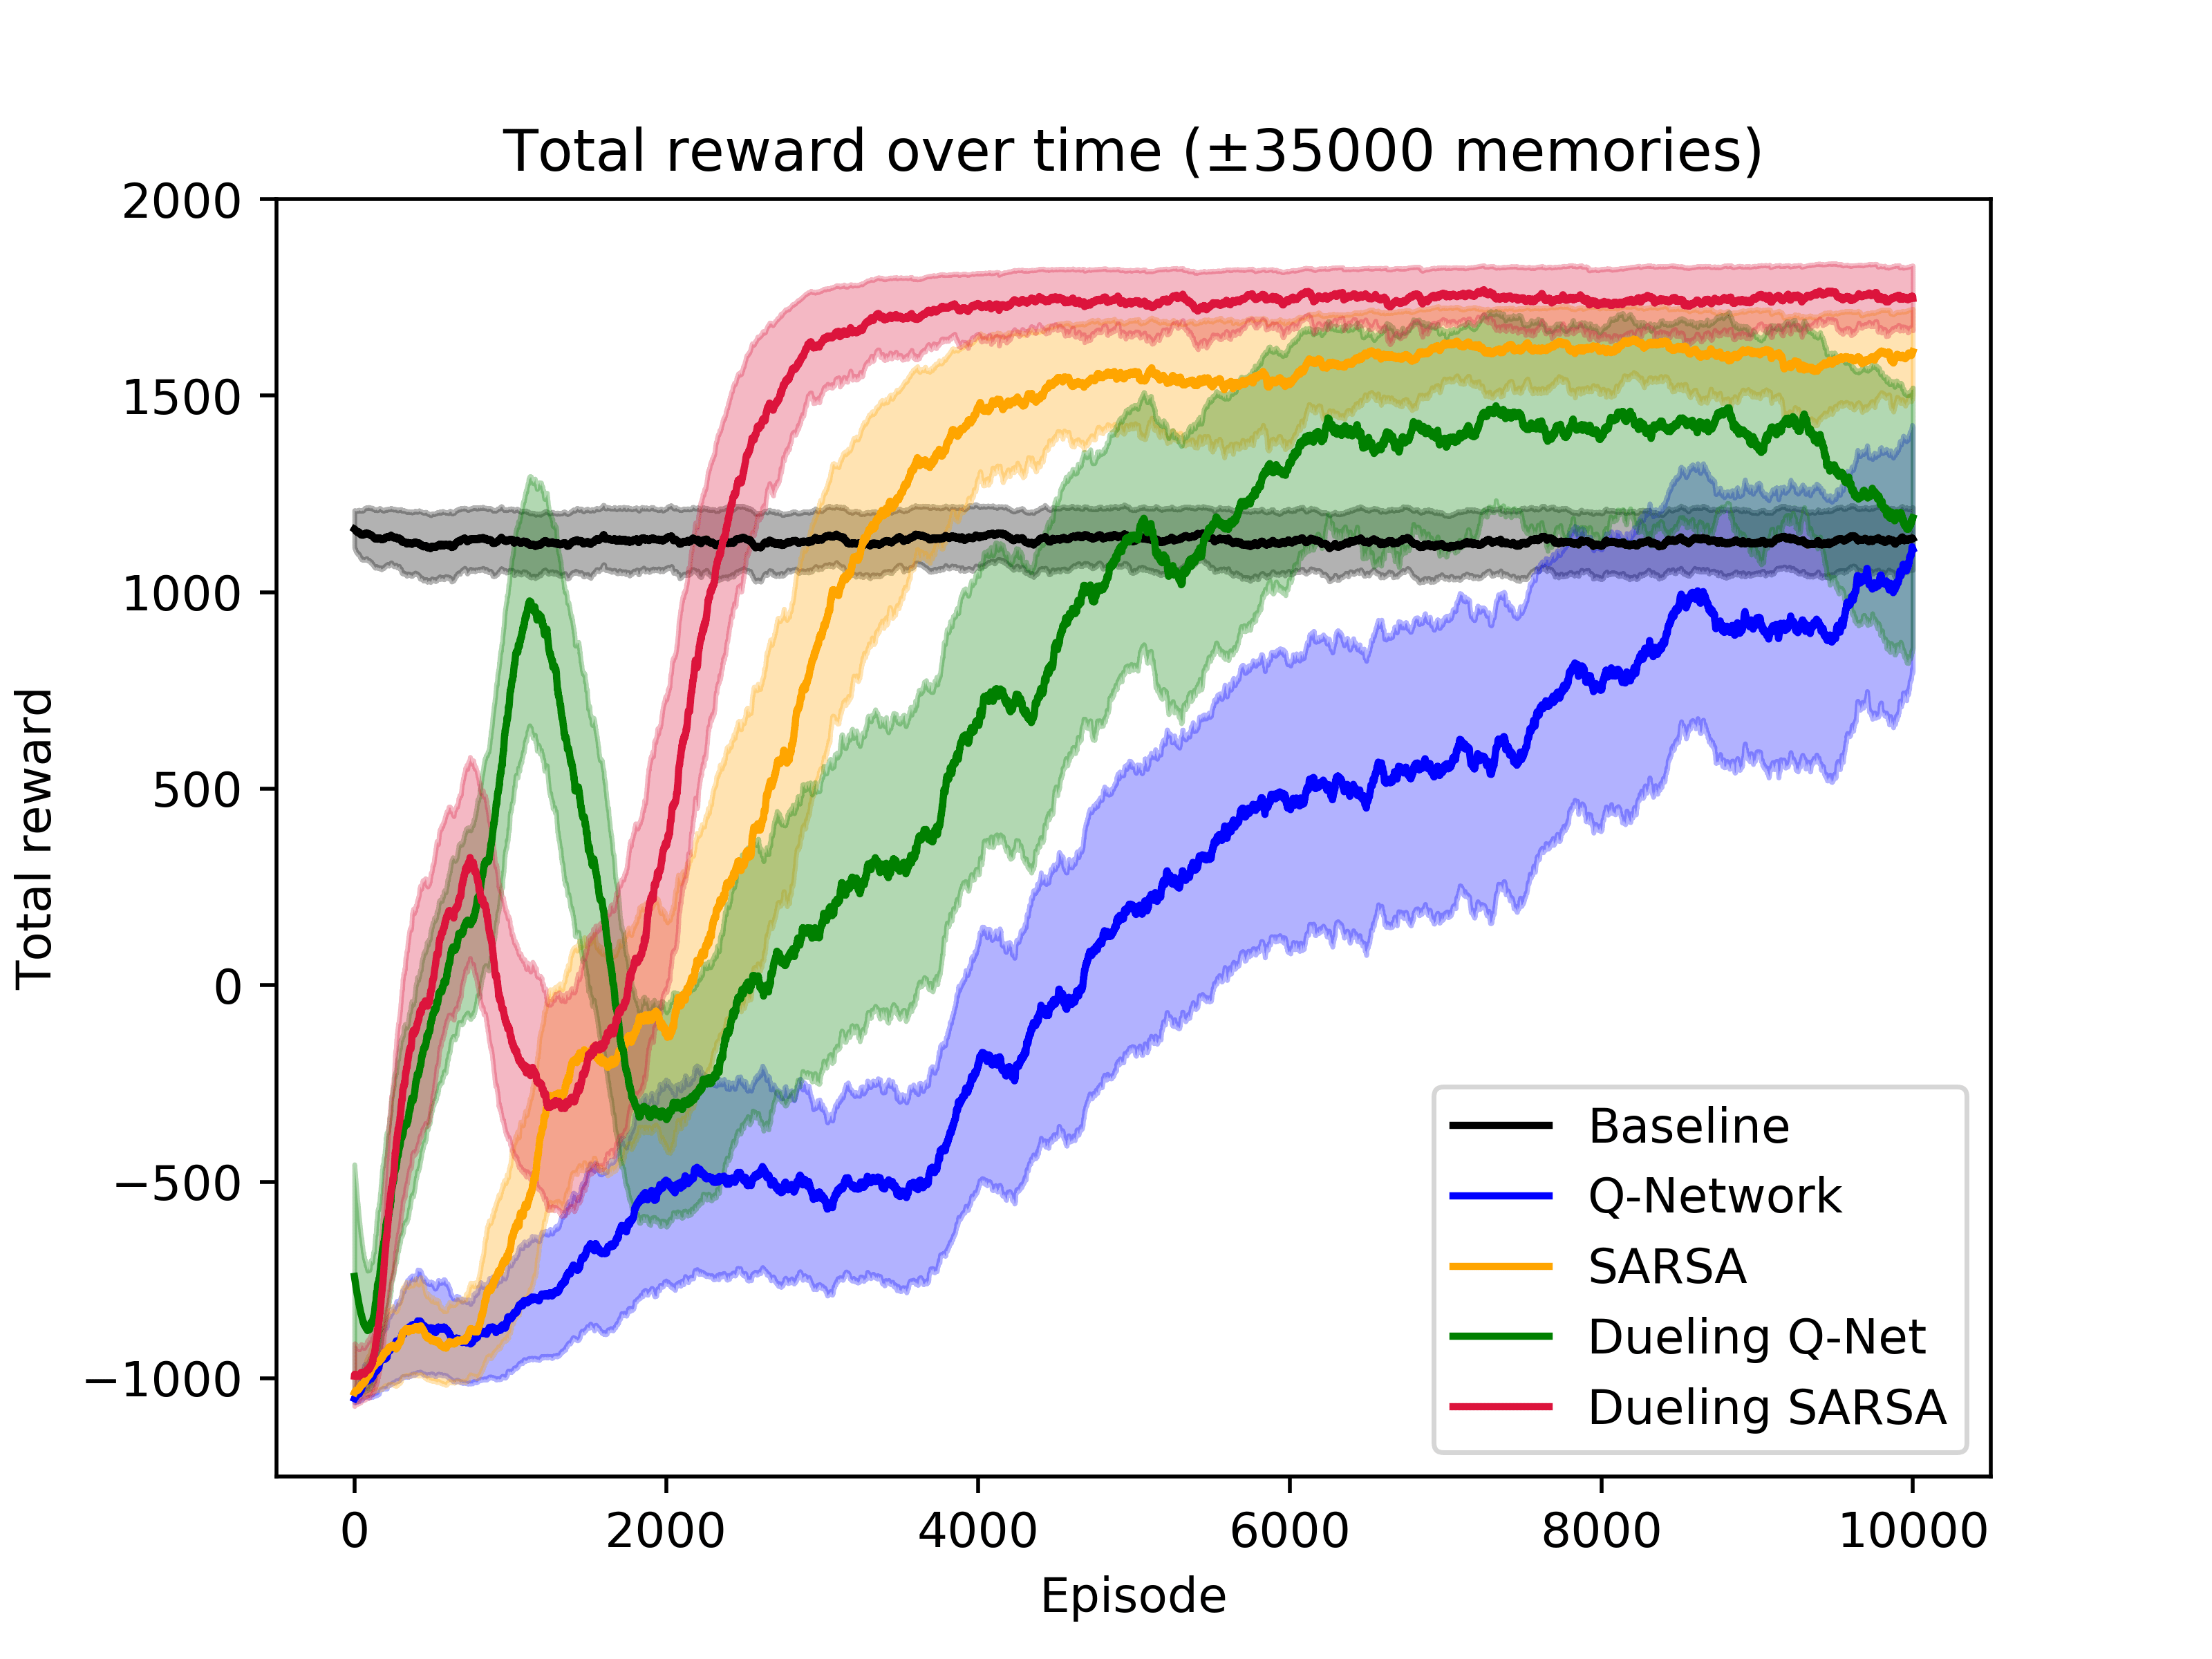
\includegraphics[width=\linewidth]{img/results/10-sized/total_rewards_1000m-min.png}
    \caption{10-run averages given 1000 episodes of demonstration data.}
    \label{fig:10sized-1000mem}
\end{figure}
% TABLES 10-sized
\begin{table}[H]
\begin{tabular}{|l|l|l|l|}
\hline
\textbf{Algorithm} & \textbf{\begin{tabular}[c]{@{}l@{}}Average\\ Reward\end{tabular}} & \textbf{\begin{tabular}[c]{@{}l@{}}Std.\\ Error\end{tabular}} & \textbf{\begin{tabular}[c]{@{}l@{}}Best\\ Reward\end{tabular}} \\ \hline
Baseline & 1129 & 1.9 & 1387 \\ \hline
Q-Network & 221 & 4.2 & 715 \\ \hline
SARSA & 132 & 3.9 & 563 \\ \hline
\begin{tabular}[c]{@{}l@{}}Dueling\\ Q-Network\end{tabular} & 956 & 4.1 & 1335 \\ \hline
\begin{tabular}[c]{@{}l@{}}Dueling\\ SARSA\end{tabular} & 241 & 2.6 & 582 \\ \hline
\end{tabular}
    \caption{Averages of the last 2500 episodes given 0 episodes of demonstation data.}
    \label{tab:10sized-0mem}
\end{table}
\begin{table}[H]
\begin{tabular}{|l|l|l|l|}
\hline
\textbf{Algorithm} & \textbf{\begin{tabular}[c]{@{}l@{}}Average\\ Reward\end{tabular}} & \textbf{\begin{tabular}[c]{@{}l@{}}Std.\\ Error\end{tabular}} & \textbf{\begin{tabular}[c]{@{}l@{}}Best\\ Reward\end{tabular}} \\ \hline
Baseline & 1129 & 1.9 & 1387 \\ \hline
Q-Network & 878 & 7.5 & 1758 \\ \hline
SARSA & 776 & 4.7 & 1292 \\ \hline
\begin{tabular}[c]{@{}l@{}}Dueling\\ Q-Network\end{tabular} & 521 & 6.8 & 1535 \\ \hline
\begin{tabular}[c]{@{}l@{}}Dueling\\ SARSA\end{tabular} & 1031 & 3.4 & 1312 \\ \hline
\end{tabular}
    \caption{Averages of the last 2500 episodes given 100 episodes of demonstation data.}
    \label{tab:10sized-100mem}
\end{table}
\begin{table}[H]
\begin{tabular}{|l|l|l|l|}
\hline
\textbf{Algorithm} & \textbf{\begin{tabular}[c]{@{}l@{}}Average\\ Reward\end{tabular}} & \textbf{\begin{tabular}[c]{@{}l@{}}Std.\\ Error\end{tabular}} & \textbf{\begin{tabular}[c]{@{}l@{}}Best\\ Reward\end{tabular}} \\ \hline
Baseline & 1129 & 1.9 & 1387 \\ \hline
Q-Network & 907 & 6.7 & 1696 \\ \hline
SARSA & 1607* & 2.8 & 1748 \\ \hline
\begin{tabular}[c]{@{}l@{}}Dueling\\ Q-Network\end{tabular} & 1369* & 5.5 & 1826 \\ \hline
\begin{tabular}[c]{@{}l@{}}Dueling\\ SARSA\end{tabular} & 1745* & 2.5 & 1860 \\ \hline
\end{tabular}
    \caption{Averages of the last 2500 episodes given 1000 episodes of demonstation data.}
    \label{tab:10sized-1000mem}
\end{table}
%FORMER 10-sized RESULTS
In Figures \ref{fig:10sized-0mem}, \ref{fig:10sized-100mem} and \ref{fig:10sized-1000mem} we see the three cases where the simulation consists of a grid of 10-by-10 cells and the algorithms are given 0, 100 or 1000 episodes of demonstration data respectively.

Firstly, in Figure \ref{fig:10sized-0mem} we see that all algorithms struggle to beat the baseline algorithm. Only the Dueling Q-Networks is able to come near. It offers a greatly increased learning speed and is able to sustain a higher maximum performance level. The other three algorithm perform similarly to each other, but noticeable worse than Dueling Q-Networks.

Secondly, in Figure \ref{fig:10sized-100mem} we see the performance of all algorithms come together. The Dueling Q-Networks which performed better than the others before, has now lost its edge and is now the worst performer. The performance of Q-Networks greatly increases when given $\pm 3500$ memories compared to none. It surpasses the baseline algorithm temporarily. SARSA and Dueling SARSA do not stand out, but also increased their performances given more memories than before.

Lastly, in Figure \ref{fig:10sized-1000mem} we see each algorithm perform differently. The Q-Network loses performance compared to the previous configuration, but still performs better than when no memories were given. The Dueling Q-Network did not improve its performance with $\pm 35000$ memories and shows a peculiar peak near the 1000th episode. SARSA has increased its performance once again and now beats the baseline algorithm. The same holds for Dueling SARSA which outperforms SARSA. Dueling SARSA shows the same, yet smaller, peak like Dueling Q-Networks. The two algorithms incorporating SARSA offer a noticeably lower standard error.

%FORMER 10-sized DISCUSSION
The results show that all algorithms perform at least reasonably well and respond very differently and sometimes uniquely to the demonstration data given at the start of the training process. Q-Networks performed best with 100 episodes of memories while the performance of Dueling Q-Networks was less dependent on the memories. The latter also showed to have a large spike in performance near the 1000th episode. This is probably due to the large amount of memories it was given. In this way, the algorithm has very few chances to make mistakes and learn from those transitions during its exploration phase. It focuses too much on the demonstrated behaviour and is hindered in trying out actions to explore consequences. This explanation can also hold for why the Q-Network performs worse with 1000 episodes of memories.
% re-read the email he sent, try to understand what he meant about the peak

SARSA showed to be one of the most consistent and trustworthy algorithms in terms of its response to the memories. In essence, more memories meant a higher sustained performance level. However, the speed at which it learned was decreased. This may also be due to the same reason mentioned; large amounts of memories hinder the algorithms exploration abilities. More memories also showed to have another positive effect on SARSA, namely its standard error. Higher performance levels came with lower standard errors. The general stability of SARSA compared to Q-Learning can be explained, as mentioned in Section \ref{sec:ql_sarsa}, by the fact that, because it is an on-policy algorithm, we effectively remove one of the three elements of the deadly triad. 

We found that combining Dueling Q-Networks and SARSA into Dueling SARSA resulted in the overall best performer, especially in high memory scenarios. It inherits the best of both worlds; the learning speed from the former, and the performance and consistency from the latter. The algorithm also inherited the performance peak from the Dueling Q-Networks, albeit not as high and slightly earlier. We estimate the maximum possible reward for an algorithm to achieve to be $\pm$1850, since it varies due to the random starting position of the agent. In Table \ref{tab:10sized-1000mem}, we see the algorithms has no problem achieving that maximum reward and having a average reward close to it. Moreover, its standard error there is similar to the baseline algorithm, which is impressive since the baseline is a hard-coded solution.

Tables \ref{tab:10sized-0mem} through \ref{tab:10sized-1000mem} show us that out of the 12 scenarios, only three times an algorithm was able to achieve an average reward higher than the baseline. All three occurred in the setting where 1000 episodes of memories were given. The Q-Network stands out as being the only one with an average reward lower than the baseline.




\subsection{14-by-14 simulations}
% FIGURES 14-sized
\begin{figure}[H]
    \centering
    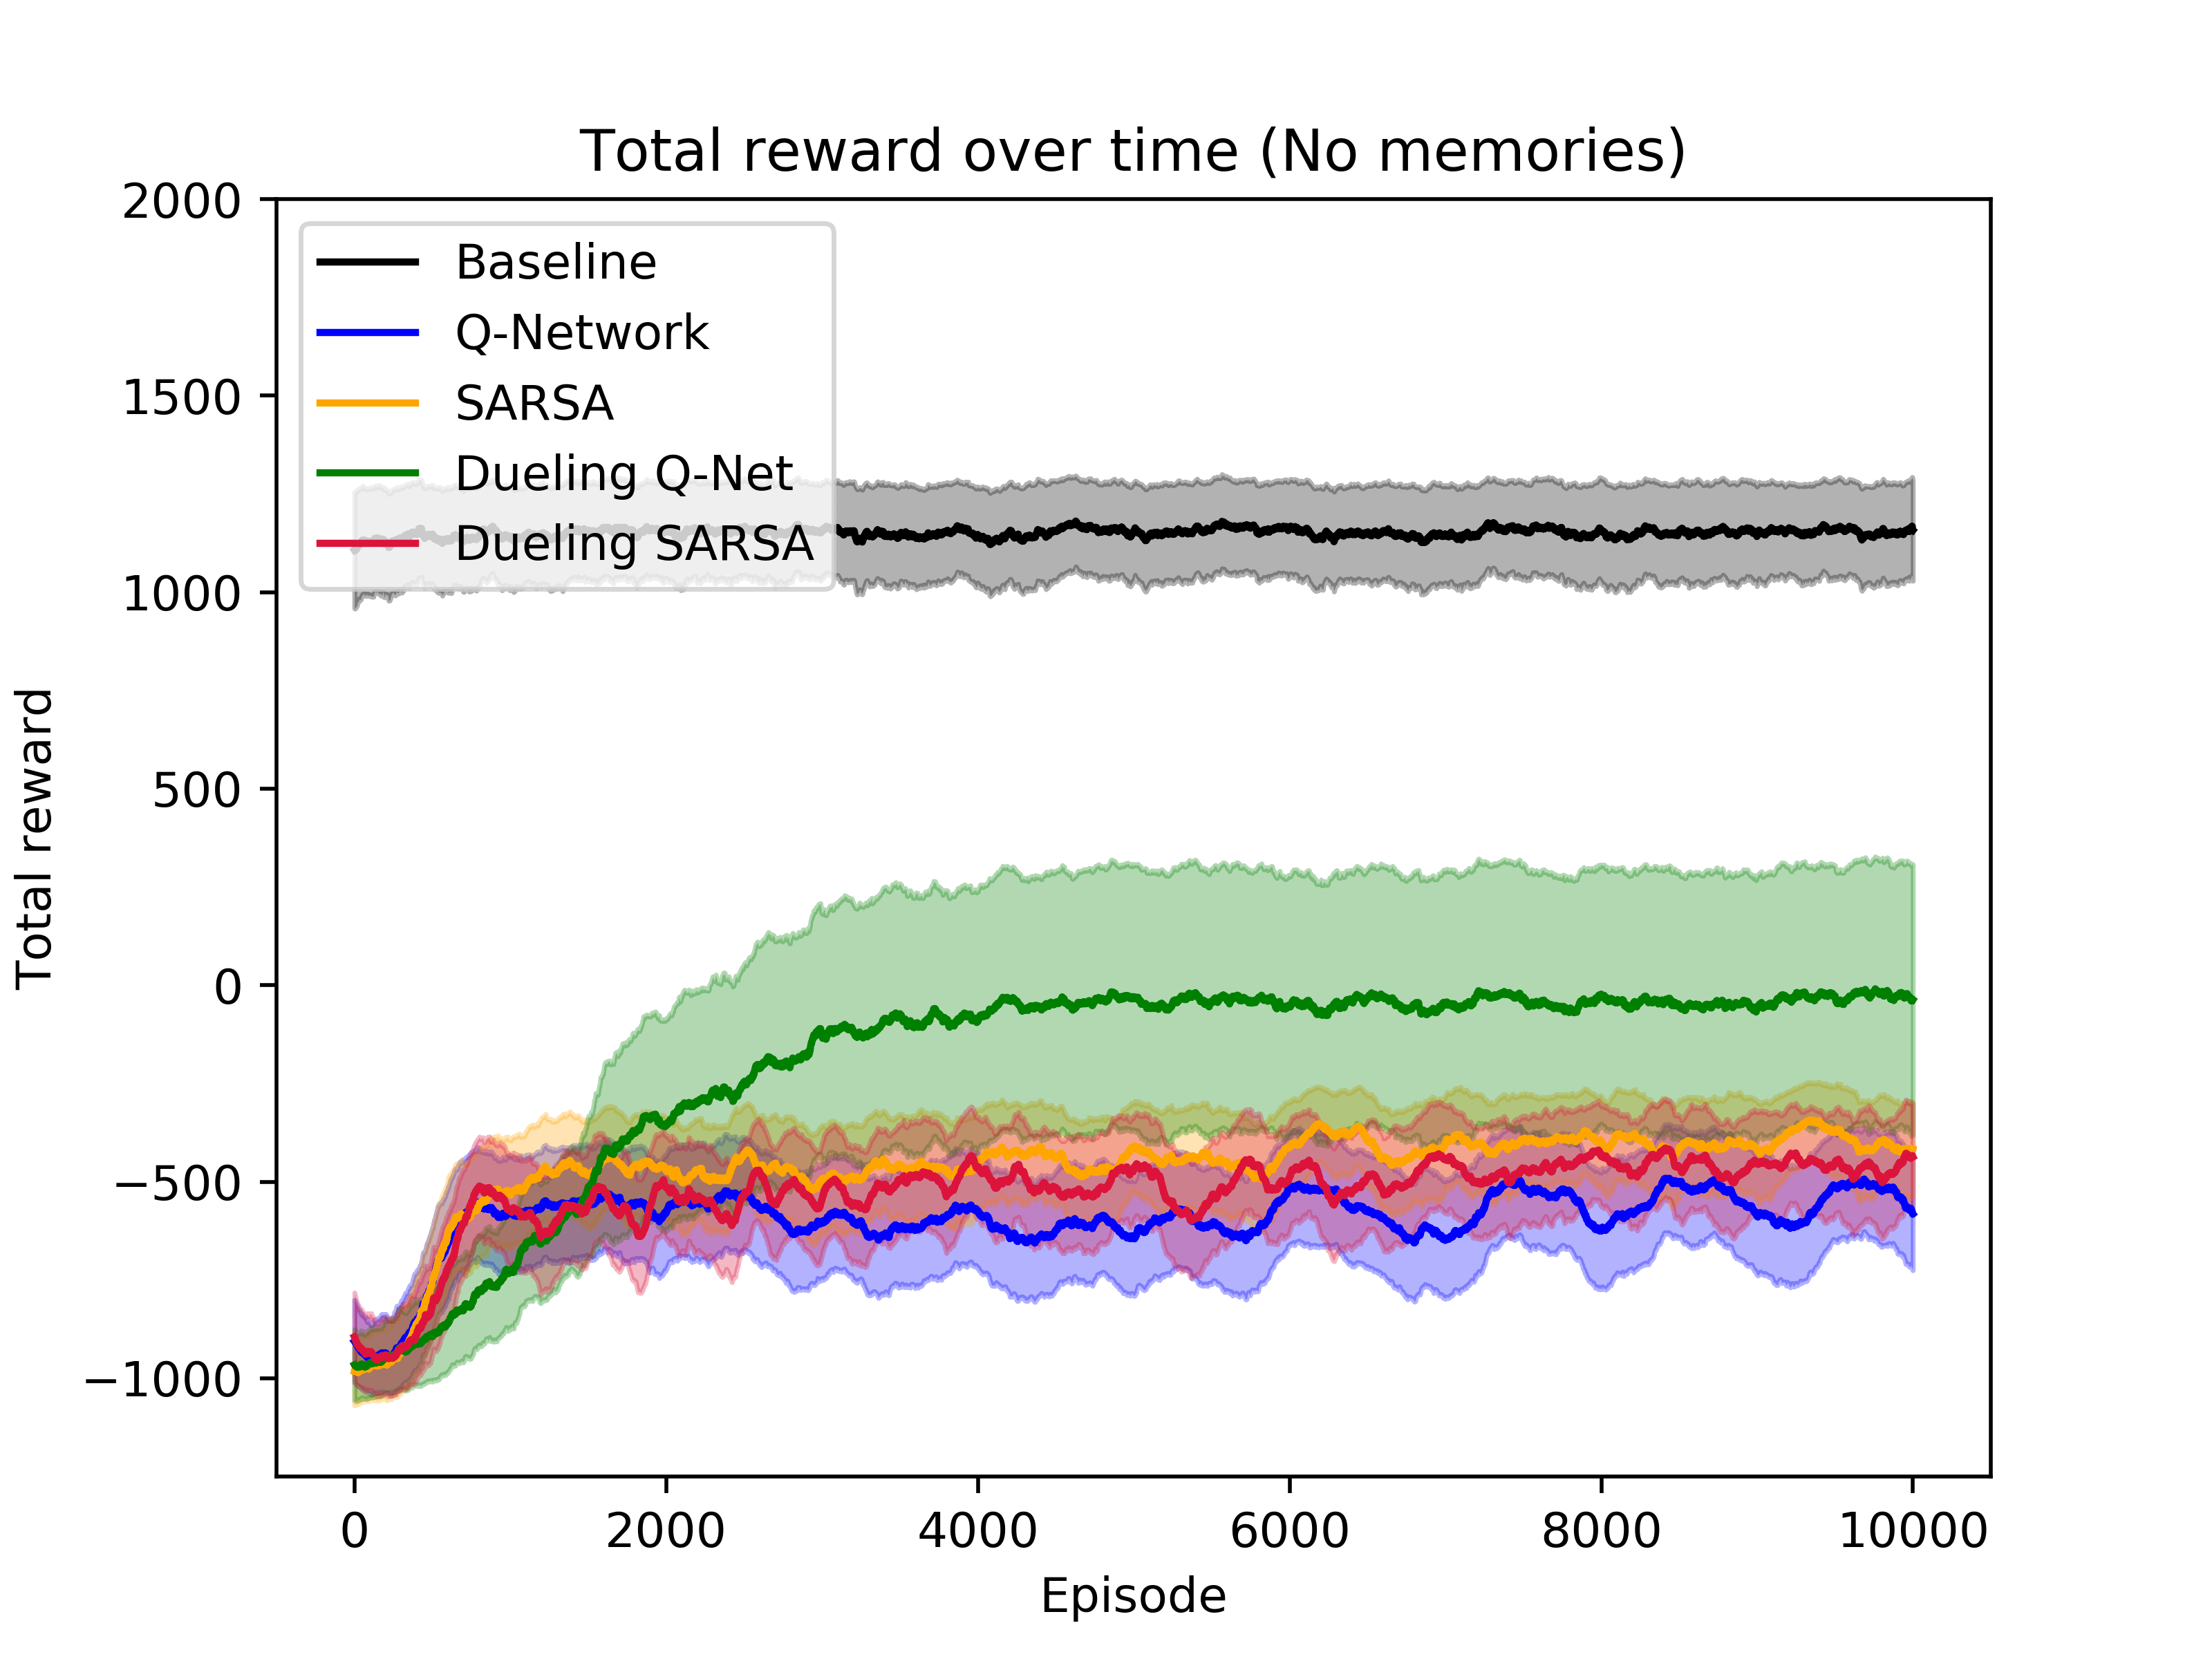
\includegraphics[width=\linewidth]{img/results/14-sized/total_rewards_0m-min.png}
    \caption{10-run averages given 0 episodes of demonstration data.}
    \label{fig:14sized-0mem}
\end{figure}
\begin{figure}[H]
    \centering
    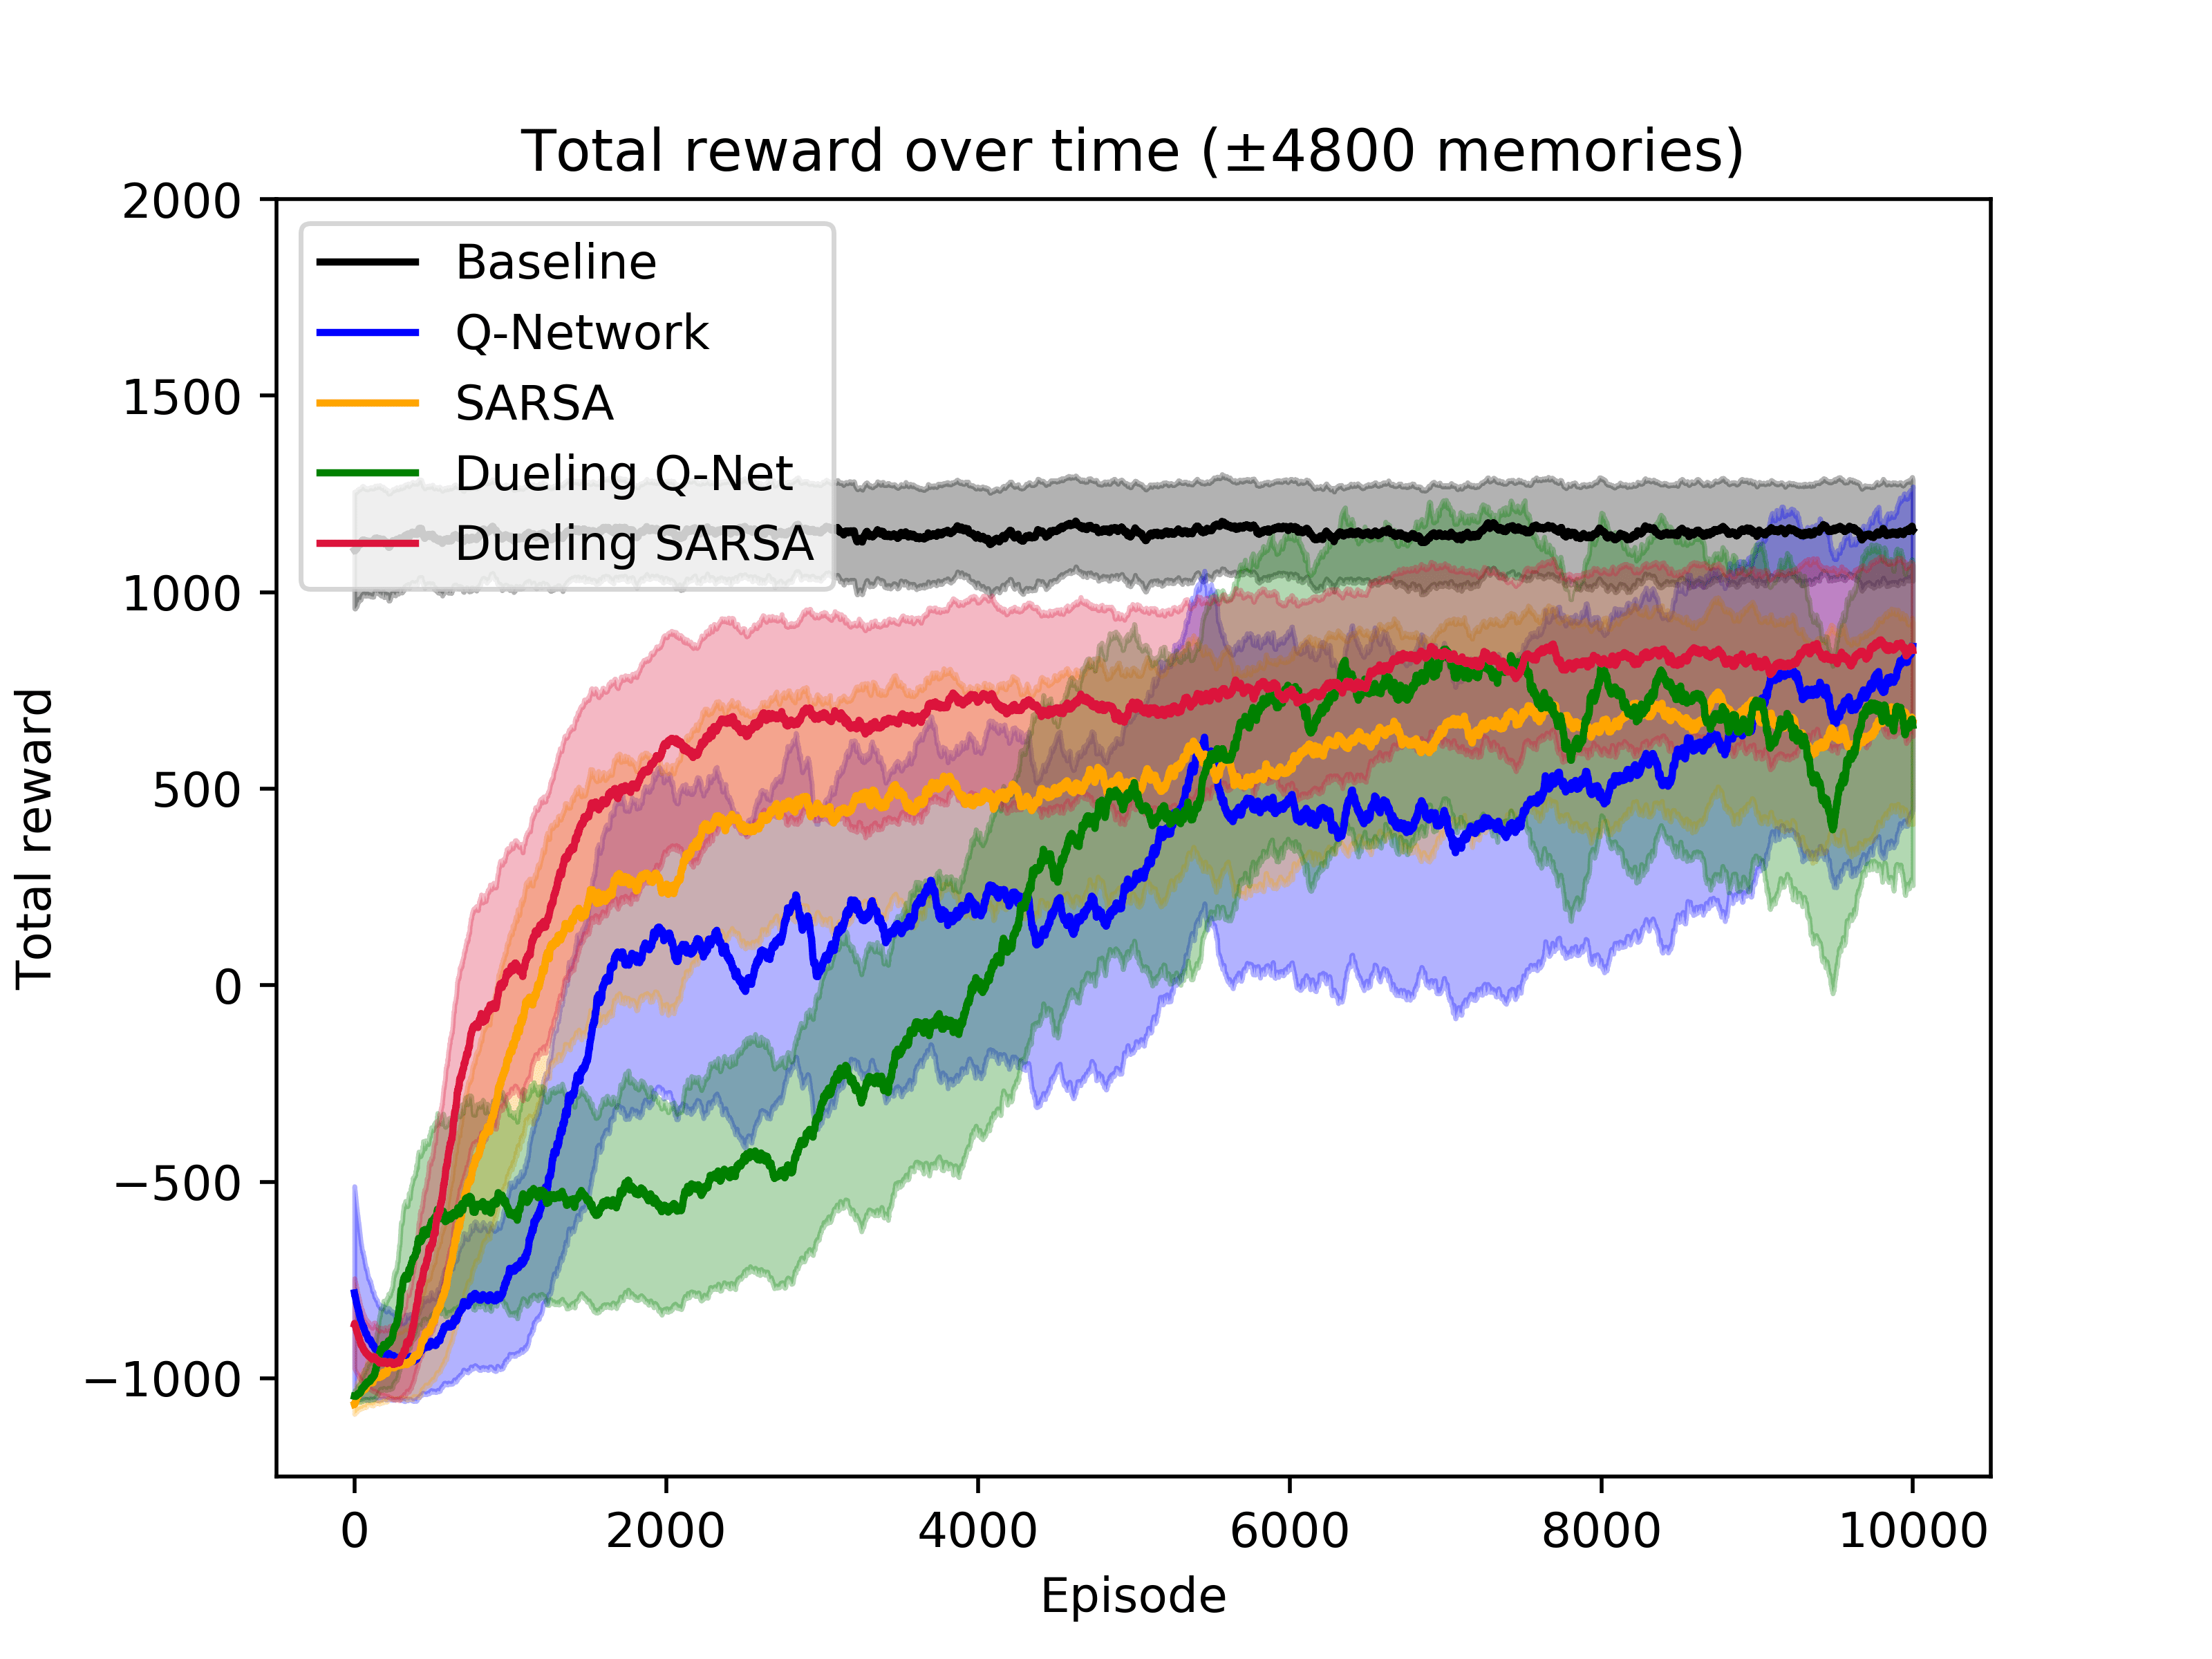
\includegraphics[width=\linewidth]{img/results/14-sized/total_rewards_100m-min.png}
    \caption{10-run averages given 100 episodes of demonstration data.}
    \label{fig:14sized-100mem}
\end{figure}
\begin{figure}[H]
    \centering
    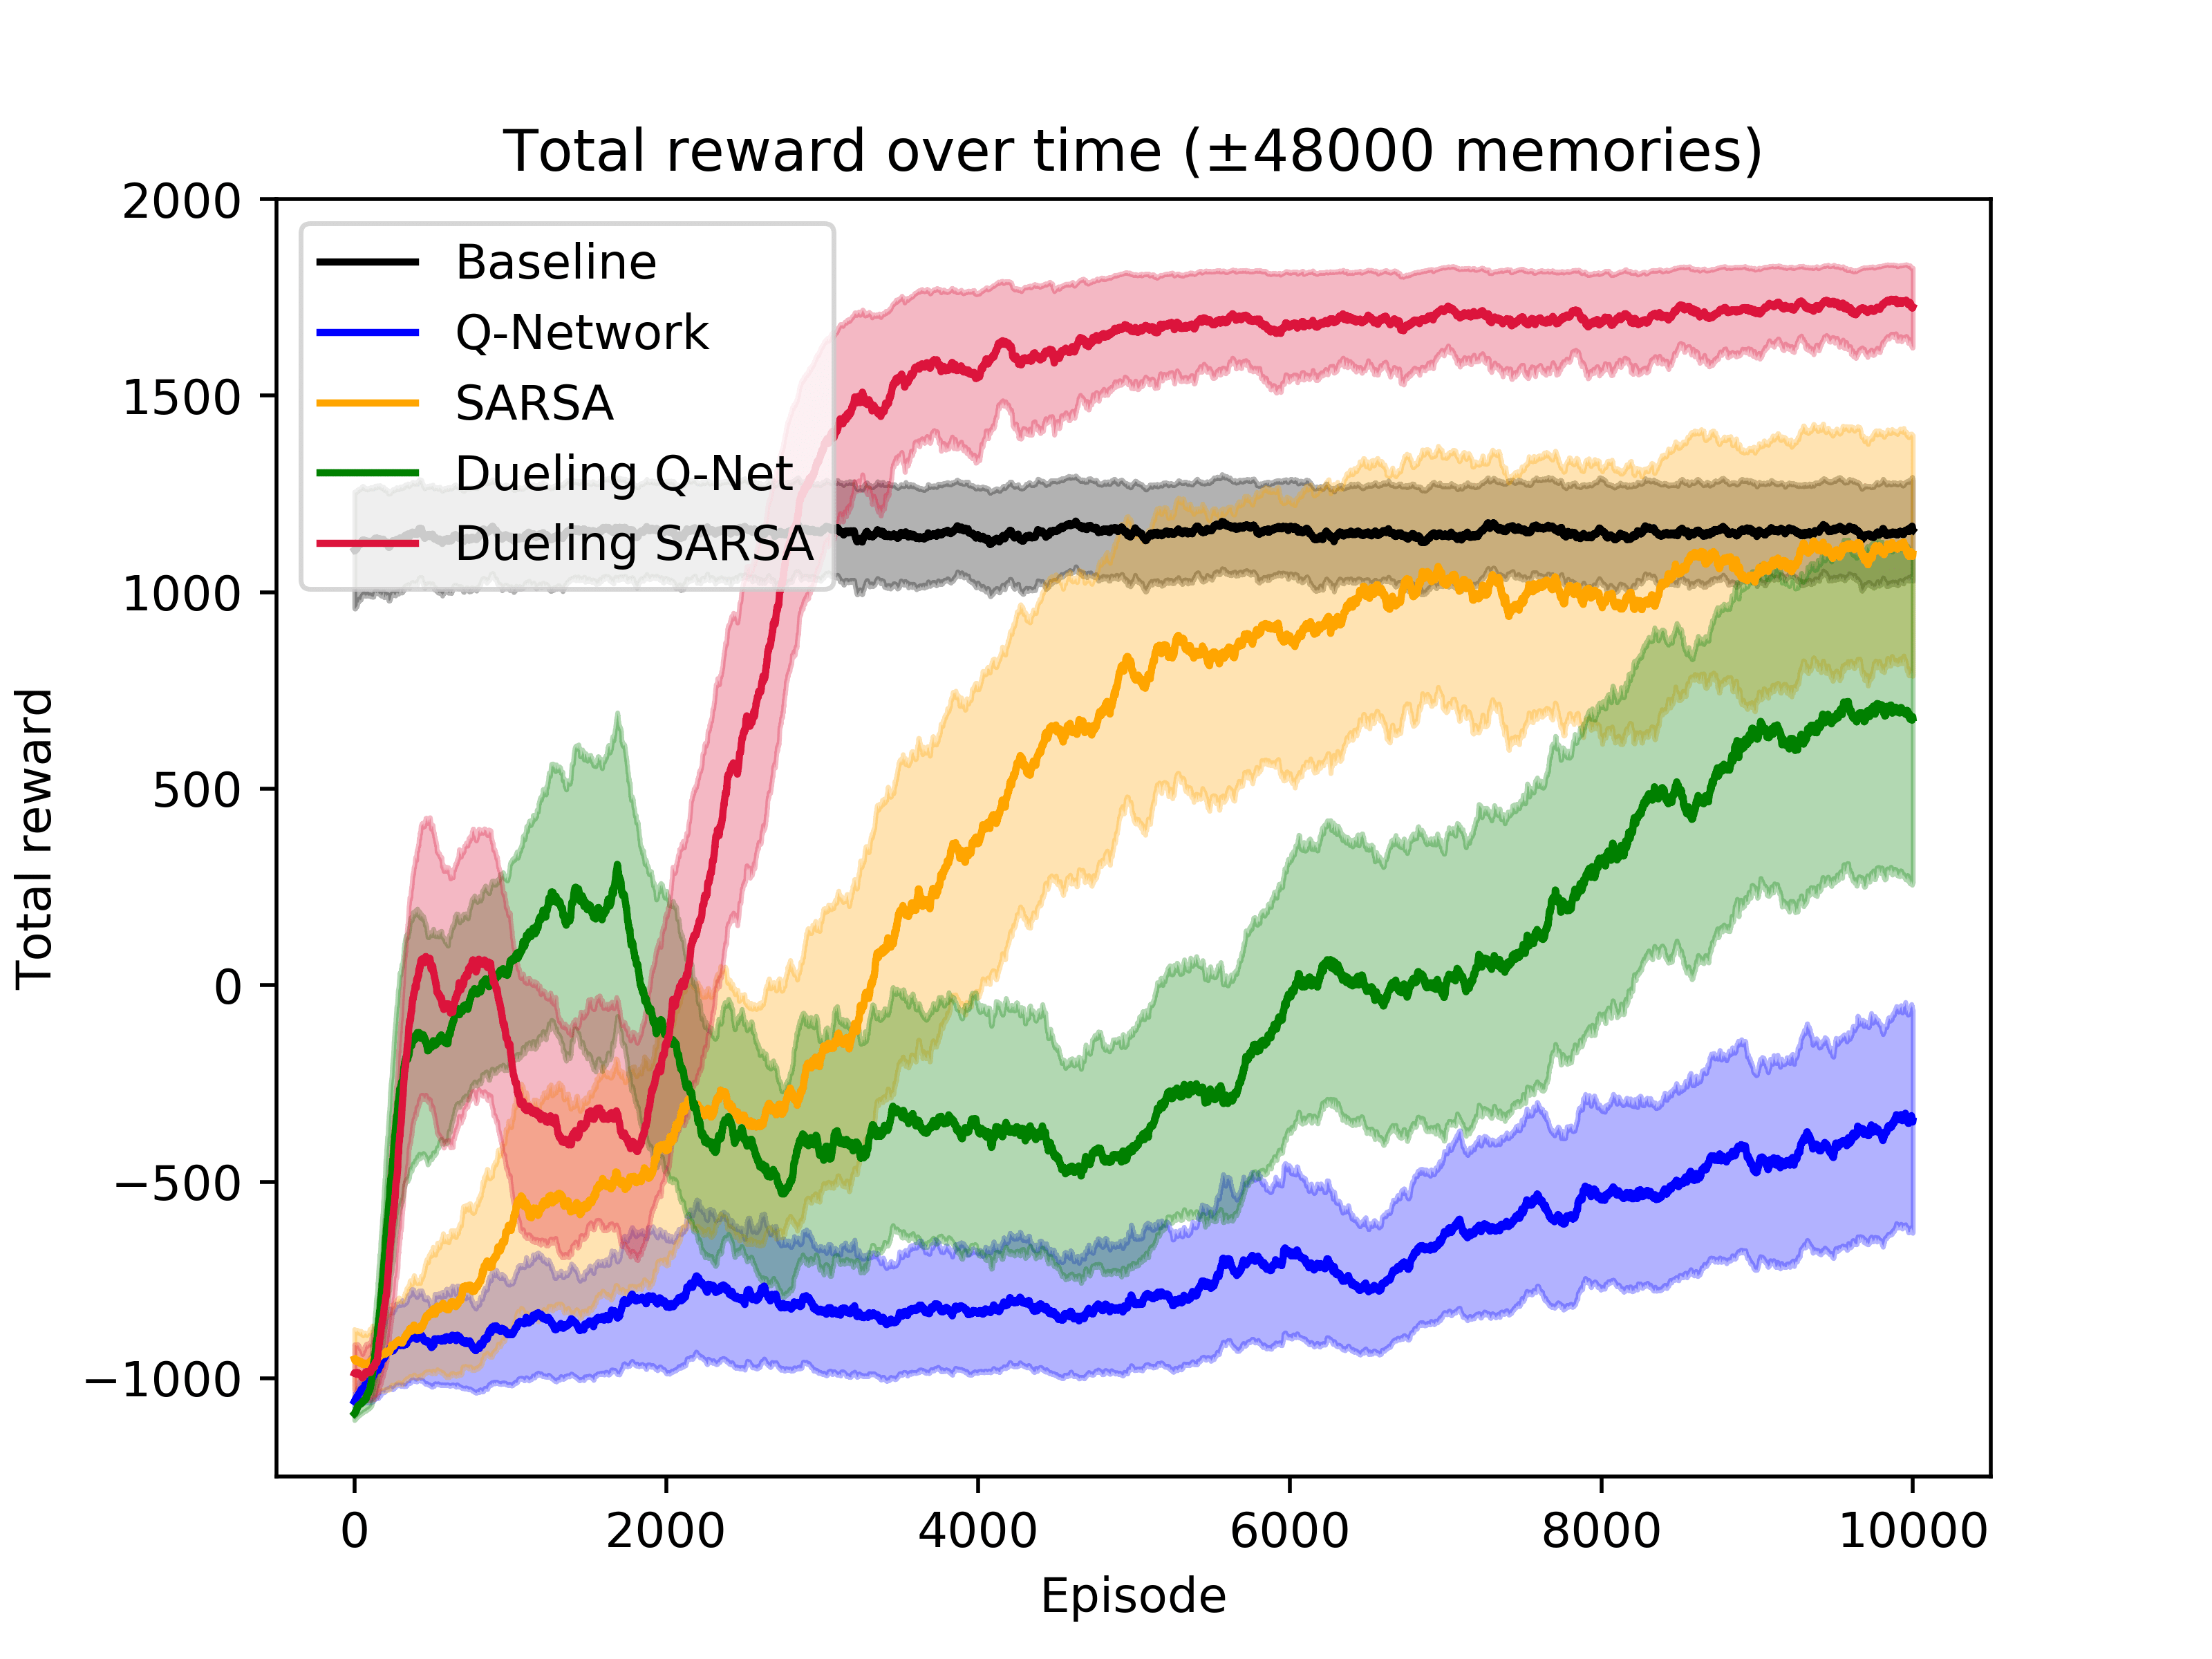
\includegraphics[width=\linewidth]{img/results/14-sized/total_rewards_1000m-min.png}
    \caption{10-run averages given 1000 episodes of demonstration data.}
    \label{fig:14sized-1000mem}
\end{figure}
% TABLES 14-sized
\begin{table}[H]
\begin{tabular}{|l|l|l|l|}
\hline
\textbf{Algorithm} & \textbf{\begin{tabular}[c]{@{}l@{}}Average\\ Reward\end{tabular}} & \textbf{\begin{tabular}[c]{@{}l@{}}Std.\\ Error\end{tabular}} & \textbf{\begin{tabular}[c]{@{}l@{}}Best\\ Reward\end{tabular}} \\ \hline
Baseline & 1152 & 2.8 & 1513 \\ \hline
Q-Network & -550 & 2.9 & -139 \\ \hline
SARSA & -398 & 2.4 & -92 \\ \hline
\begin{tabular}[c]{@{}l@{}}Dueling\\ Q-Network\end{tabular} & -40 & 3.0 & 349 \\ \hline
\begin{tabular}[c]{@{}l@{}}Dueling\\ SARSA\end{tabular} & -455 & 2.6 & -44 \\ \hline
\end{tabular}
    \caption{Averages of the last 2500 episodes given 0 episodes of demonstation data.}
    \label{tab:14sized-0mem}
\end{table}
\begin{table}[H]
\begin{tabular}{|l|l|l|l|}
\hline
\textbf{Algorithm} & \textbf{\begin{tabular}[c]{@{}l@{}}Average\\ Reward\end{tabular}} & \textbf{\begin{tabular}[c]{@{}l@{}}Std.\\ Error\end{tabular}} & \textbf{\begin{tabular}[c]{@{}l@{}}Best\\ Reward\end{tabular}} \\ \hline
Baseline & 1152 & 2.8 & 1513 \\ \hline
Q-Network & 652 & 7.0 & 169 \\ \hline
SARSA & 670 & 5.3 & 1275 \\ \hline
\begin{tabular}[c]{@{}l@{}}Dueling\\ Q-Network\end{tabular} & 667 & 7.8 & 1748 \\ \hline
\begin{tabular}[c]{@{}l@{}}Dueling\\ SARSA\end{tabular} & 836 & 4.1 & 1249 \\ \hline
\end{tabular}
    \caption{Averages of the last 2500 episodes given 100 episodes of demonstation data.}
    \label{tab:14sized-100mem}
\end{table}
\begin{table}[H]
\begin{tabular}{|l|l|l|l|}
\hline
\textbf{Algorithm} & \textbf{\begin{tabular}[c]{@{}l@{}}Average\\ Reward\end{tabular}} & \textbf{\begin{tabular}[c]{@{}l@{}}Std.\\ Error\end{tabular}} & \textbf{\begin{tabular}[c]{@{}l@{}}Best\\ Reward\end{tabular}} \\ \hline
Baseline & 1152 & 2.8 & 1513 \\ \hline
Q-Network & -459 & 5.0 & 411 \\ \hline
SARSA & 1057 & 5.6 & 1626 \\ \hline
\begin{tabular}[c]{@{}l@{}}Dueling\\ Q-Network\end{tabular} & 522 & 7.7 & 1534 \\ \hline
\begin{tabular}[c]{@{}l@{}}Dueling\\ SARSA\end{tabular} & 1713* & 3.0 & 1846 \\ \hline
\end{tabular}
    \caption{Averages of the last 2500 episodes given 1000 episodes of demonstation data.}
    \label{tab:14sized-1000mem}
\end{table}
%FORMER 14-sized RESULTS
In Figure \ref{fig:14sized-0mem}, \ref{fig:14sized-100mem} and \ref{fig:14sized-1000mem} we see the three cases where the simulation has a grid size of 14-by-14 and the algorithms are given 0, 100 or 1000 episodes of demonstation data.

Firstly, in Figure \ref{fig:14sized-0mem} we see results comparable to Figure \ref{fig:10sized-0mem}, however the performance difference of Dueling Q-Networks compared to the rest has decreased. The best performing algorithm here does not come close to the performance of the baseline.

Secondly, in Figure \ref{fig:14sized-100mem} we see results similar to Figure \ref{fig:10sized-100mem}, but no algorithm is able to beat the baseline like Q-Networks was able to before.

Lastly, in Figure \ref{fig:14sized-1000mem} we once again see results comparable to Figure \ref{fig:10sized-1000mem}, however only Dueling SARSA is now able to beat the baseline algorithm. SARSA is able to perform at the same level as the baseline in the end. The (Dueling) Q-Networks do not offer good performance, but Dueling Q-Networks does outperform Q-Networks.

%FORMER 14-sized DISCUSSION
When switching to a simulation consisting of a square grid of size 14 instead of 10, we see the algorithms struggle a lot more in general. Since we use vision grids, this nearly doubles the amount of inputs from 300 to 588. The relatively small hidden layer used seems to struggle to properly learn and process all information. The number of episodes that the algorithm was allowed to learn for was also kept constant which could explain the low overall performances.

When the algorithms are not given any memories the Dueling Q-Networks is still able to perform better than the rest, but it achieves similar scores to the worst performers in the 10-by-10 simulation. Q-Networks, SARSA and Dueling SARSA seem to barely improve at all. When given 100 or 1000 episodes of memories the Dueling Q-Network improves in both cases, but does not achieve the same levels of performance. The Q-Network shows the same behaviour as before as it performs best with the medium amount of memories given and drops that advantage when given a high amount. This algorithm is also not able to solve the problem. Both Q-Network and Dueling Q-Networks fail to solve the problem and beat the baseline in all cases.

SARSA is still very receptive to memories with its best performance being the scenario where $\pm 48000$ memories were given. Here it is the only algorithm so far that is able to match the baseline algorithm. The only algorithm that is able to consistently beat it is Dueling SARSA in the high memory scenario. It shows performance very similar to the 10-by-10 simulation. The only difference is that it tops out later and suffers from a slightly higher standard error.

One other interesting thing to mention is that in the 14-by-14 simulation Both Dueling Q-Networks and Dueling SARSA show a peak in performance at the start of the learning process as well. While the peak is now not as high, both algorithms have a peak of roughly the same size. The peaks are more spread out and Dueling SARSA's peak still happens earlier. In the 10-by-10 simulation both algorithms managed to quickly regain performance and continue learning after this peak, while in the 14-by-14 simulation only Dueling SARSA is able to continue learning properly.

To conclude this section, we can look at the figures with an asterisk (*) in Tables \ref{tab:10sized-0mem} through \ref{tab:14sized-1000mem}. These are the cases where the average score of the last 2500 episodes of an algorithm was greater than the same average of the baseline. In the 24 algorithm/memory/size combinations, this happened only four times. Two of which were performed by the Dueling SARSA algorithm. With the highest amount of memories it was the only algorithm to solve the task successfully on both the 10-by-10 and 14-by-14 simulations. When looking at just the scenario where the algorithms were given the maximum amount of memories on a 10-by-10 simulation, two other algorithms were able to succeed: Dueling Q-Networks and SARSA. This rhymes nicely with the expectation that combining these two algorithms into Dueling SARSA makes it inherit the best of both worlds.